\chapter{Flujos y cortes}

En este capítulo, nos centraremos en los dos problemas siguientes:

\begin{itemize}
    \item \key{Encontrar un flujo máximo}: ¿cuál es la máxima cantidad
          de flujo que podemos enviar de un nodo a otro?
    \item \key{Encontrar un corte mínimo}: ¿cuál es un conjunto de
          aristas de peso total mínimo que separe dos nodos del grafo?
\end{itemize}

La entrada para estos dos problemas es un grafo dirigido y ponderado que
contiene dos nodos especiales: la \emph{fuente} es un nodo sin aristas
entrantes, y el \emph{pozo} es un nodo sin aristas salientes.

Por ejemplo, veamos el siguiente grafo donde el nodo 1 es la fuente
y el nodo 6 es el pozo:

\begin{center}
    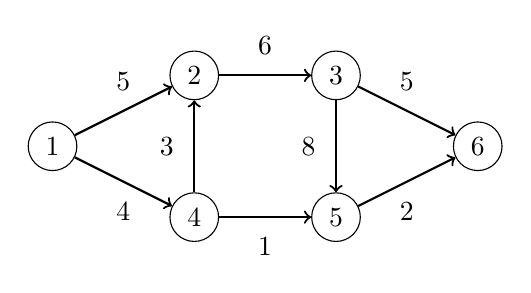
\begin{tikzpicture}[scale=0.9]
        \node[draw, circle] (1) at (1,2) {$1$};
        \node[draw, circle] (2) at (3,3) {$2$};
        \node[draw, circle] (3) at (5,3) {$3$};
        \node[draw, circle] (4) at (7,2) {$6$};
        \node[draw, circle] (5) at (3,1) {$4$};
        \node[draw, circle] (6) at (5,1) {$5$};
        \path[draw,thick,->] (1) -- node[font=\small,label=5] {} (2);
        \path[draw,thick,->] (2) -- node[font=\small,label=6] {} (3);
        \path[draw,thick,->] (3) -- node[font=\small,label=5] {} (4);
        \path[draw,thick,->] (1) -- node[font=\small,label=below:4] {} (5);
        \path[draw,thick,->] (5) -- node[font=\small,label=below:1] {} (6);
        \path[draw,thick,->] (6) -- node[font=\small,label=below:2] {} (4);
        \path[draw,thick,<-] (2) -- node[font=\small,label=left:3] {} (5);
        \path[draw,thick,->] (3) -- node[font=\small,label=left:8] {} (6);
    \end{tikzpicture}
\end{center}

\subsubsection{Flujo máximo}

\index{flujo máximo}

En el problema de \key{flujo máximo}, nuestra tarea es enviar tanto
flujo como sea posible desde la fuente hacia el pozo. El peso de cada
arista es una capacidad que restringe el flujo que puede pasar por ella.
En cada nodo intermedio, el flujo entrante y saliente debe ser igual.

Por ejemplo, el máximo tamaño de un flujo en el grafo de ejemplo es 7.
La siguiente imagen muestra cómo podríamos enviar el flujo:

\begin{center}
    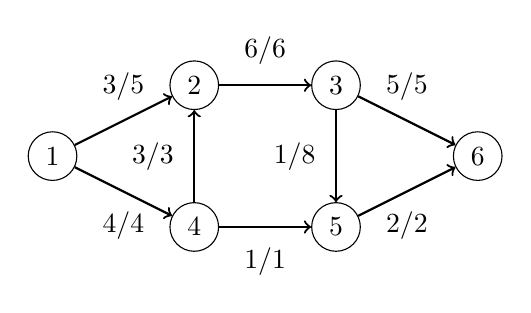
\begin{tikzpicture}[scale=0.9]
        \node[draw, circle] (1) at (1,2) {$1$};
        \node[draw, circle] (2) at (3,3) {$2$};
        \node[draw, circle] (3) at (5,3) {$3$};
        \node[draw, circle] (4) at (7,2) {$6$};
        \node[draw, circle] (5) at (3,1) {$4$};
        \node[draw, circle] (6) at (5,1) {$5$};
        \path[draw,thick,->] (1) -- node[font=\small,label=3/5] {} (2);
        \path[draw,thick,->] (2) -- node[font=\small,label=6/6] {} (3);
        \path[draw,thick,->] (3) -- node[font=\small,label=5/5] {} (4);
        \path[draw,thick,->] (1) -- node[font=\small,label=below:4/4] {} (5);
        \path[draw,thick,->] (5) -- node[font=\small,label=below:1/1] {} (6);
        \path[draw,thick,->] (6) -- node[font=\small,label=below:2/2] {} (4);
        \path[draw,thick,<-] (2) -- node[font=\small,label=left:3/3] {} (5);
        \path[draw,thick,->] (3) -- node[font=\small,label=left:1/8] {} (6);
    \end{tikzpicture}
\end{center}

La notación $v/k$ indica que se envía un flujo de $v$ unidades
a través de una arista cuya capacidad es de $k$ unidades. El tamaño
del flujo es de $7$, porque la fuente envía $3+4$ unidades de flujo
y el pozo recibe $5+2$ unidades de flujo. Es fácil ver que este
flujo es máximo, porque la capacidad total de las aristas que llevan
al pozo es de $7$.

\subsubsection{Corte mínimo}

\index{corte mínimo}

En el problema del \key{corte mínimo}, nuestra tarea es remover un
conjunto de nodos del grafo tal que no haya caminos desde la fuente
hacia el pozo luego de la remoción, y el peso total de las aristas
removidas sea mínimo.

El tamaño mínimo de un corte en el grafo de ejemplo es 7. Es suficiente
remover las aristas $2 \rightarrow 3$ y $4 \rightarrow 5$:

\begin{center}
    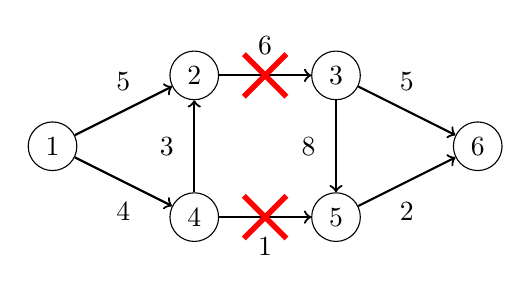
\begin{tikzpicture}[scale=0.9]
        \node[draw, circle] (1) at (1,2) {$1$};
        \node[draw, circle] (2) at (3,3) {$2$};
        \node[draw, circle] (3) at (5,3) {$3$};
        \node[draw, circle] (4) at (7,2) {$6$};
        \node[draw, circle] (5) at (3,1) {$4$};
        \node[draw, circle] (6) at (5,1) {$5$};
        \path[draw,thick,->] (1) -- node[font=\small,label=5] {} (2);
        \path[draw,thick,->] (2) -- node[font=\small,label=6] {} (3);
        \path[draw,thick,->] (3) -- node[font=\small,label=5] {} (4);
        \path[draw,thick,->] (1) -- node[font=\small,label=below:4] {} (5);
        \path[draw,thick,->] (5) -- node[font=\small,label=below:1] {} (6);
        \path[draw,thick,->] (6) -- node[font=\small,label=below:2] {} (4);
        \path[draw,thick,<-] (2) -- node[font=\small,label=left:3] {} (5);
        \path[draw,thick,->] (3) -- node[font=\small,label=left:8] {} (6);

        \path[draw=red,thick,-,line width=2pt] (4-.3,3-.3) -- (4+.3,3+.3);
        \path[draw=red,thick,-,line width=2pt] (4-.3,3+.3) -- (4+.3,3-.3);
        \path[draw=red,thick,-,line width=2pt] (4-.3,1-.3) -- (4+.3,1+.3);
        \path[draw=red,thick,-,line width=2pt] (4-.3,1+.3) -- (4+.3,1-.3);
    \end{tikzpicture}
\end{center}

Habiendo removido las aristas, no habrá ningún camino de la fuente
al pozo. El tamaño del corte es $7$, porque los pesos de las aristas
removidas son $6$ y $1$. El corte es mínimo, porque no hay forma
válida de remover aristas del grafo tal que su peso total sea
menos que $7$.

No es coincidencia que los valores del flujo máximo y del corte mínimo
sean iguales en el ejemplo anterior. Resulta que el flujo máximo y el
corte mínimo \emph{siempre} son iguales, y los conceptos son dos caras
de una misma moneda.

Ahora veremos el algoritmo de Ford--Fulkerson, que puede utilizarse
para encontrar el flujo máximo y corte mínimo de un grafo. El algoritmo
también nos ayuda a entender \emph{por qué} son de igual magnitud.

\section{Algoritmo de Ford--Fulkerson}

\index{algoritmo de Ford--Fulkerson}

El \key{algoritmo de Ford--Fulkerson} \cite{for56} encuentra el
flujo máximo en un grafo. El algoritmo comienza con un flujo vacío,
y en cada paso encuentra un camino de la fuente al pozo que genere más
flujo. Finalmente, cuando el algoritmo no pueda aumentar más el flujo,
el flujo máximo ha sido encontrado.

El algoritmo usa una representación especial del grafo donde cada
arista original tiene una arista inversa en otra dirección. El peso
de cada arista indica cuánto más flujo podríamos dirigir mediante ella.
Al comienzo del algoritmo, el peso de cada arista original es igual a
la capacidad de la arista y el peso de cada arista inversa es cero.

\newpage
La nueva representación para el grafo de ejemplo es la siguiente:

\begin{center}
    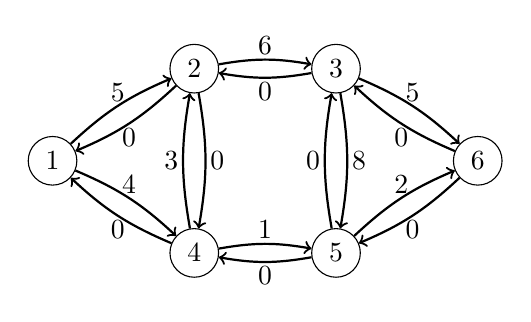
\begin{tikzpicture}[scale=0.9,label distance=-2mm]
        \node[draw, circle] (1) at (1,1.3) {$1$};
        \node[draw, circle] (2) at (3,2.6) {$2$};
        \node[draw, circle] (3) at (5,2.6) {$3$};
        \node[draw, circle] (4) at (7,1.3) {$6$};
        \node[draw, circle] (5) at (3,0) {$4$};
        \node[draw, circle] (6) at (5,0) {$5$};

        \path[draw,thick,->] (1) edge [bend left=10] node[font=\small,label=5] {} (2);
        \path[draw,thick,->] (2) edge [bend left=10] node[font=\small,label=below:0] {} (1);
        \path[draw,thick,->] (2) edge [bend left=10] node[font=\small,label=6] {} (3);
        \path[draw,thick,->] (3) edge [bend left=10] node[font=\small,label=below:0] {} (2);
        \path[draw,thick,->] (3) edge [bend left=10] node[font=\small,label=5] {} (4);
        \path[draw,thick,->] (4) edge [bend left=10] node[font=\small,label=below:0] {} (3);
        \path[draw,thick,->] (1) edge [bend left=10] node[font=\small,label=4] {} (5);
        \path[draw,thick,->] (5) edge [bend left=10] node[font=\small,label=below:0] {} (1);
        \path[draw,thick,->] (5) edge [bend left=10] node[font=\small,label=1] {} (6);
        \path[draw,thick,->] (6) edge [bend left=10] node[font=\small,label=below:0] {} (5);
        \path[draw,thick,->] (6) edge [bend left=10] node[font=\small,label=2] {} (4);
        \path[draw,thick,->] (4) edge [bend left=10] node[font=\small,label=below:0] {} (6);
        \path[draw,thick,->] (5) edge [bend left=10] node[font=\small,label=left:3] {} (2);
        \path[draw,thick,->] (2) edge [bend left=10] node[font=\small,label=right:0] {} (5);
        \path[draw,thick,->] (3) edge [bend left=10] node[font=\small,label=right:8] {} (6);
        \path[draw,thick,->] (6) edge [bend left=10] node[font=\small,label=left:0] {} (3);
    \end{tikzpicture}
\end{center}

\subsubsection{Descripción del algoritmo}

El algoritmo de Ford--Fulkerson consiste de múltiples rondas. En cada
ronda, el algoritmo encuentra un camino de la fuente al pozo tal que
cada arista en el camino tenga un peso positivo. Si hay más de un
posible camino, podemos elegir cualquiera de ellos.

Por ejemplo, supongamos que elegimos el siguiente camino:

\begin{center}
    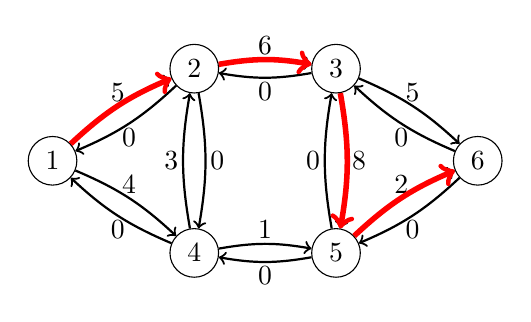
\begin{tikzpicture}[scale=0.9,label distance=-2mm]
        \node[draw, circle] (1) at (1,1.3) {$1$};
        \node[draw, circle] (2) at (3,2.6) {$2$};
        \node[draw, circle] (3) at (5,2.6) {$3$};
        \node[draw, circle] (4) at (7,1.3) {$6$};
        \node[draw, circle] (5) at (3,0) {$4$};
        \node[draw, circle] (6) at (5,0) {$5$};

        \path[draw,thick,->] (1) edge [bend left=10] node[font=\small,label=5] {} (2);
        \path[draw,thick,->] (2) edge [bend left=10] node[font=\small,label=below:0] {} (1);
        \path[draw,thick,->] (2) edge [bend left=10] node[font=\small,label=6] {} (3);
        \path[draw,thick,->] (3) edge [bend left=10] node[font=\small,label=below:0] {} (2);
        \path[draw,thick,->] (3) edge [bend left=10] node[font=\small,label=5] {} (4);
        \path[draw,thick,->] (4) edge [bend left=10] node[font=\small,label=below:0] {} (3);
        \path[draw,thick,->] (1) edge [bend left=10] node[font=\small,label=4] {} (5);
        \path[draw,thick,->] (5) edge [bend left=10] node[font=\small,label=below:0] {} (1);
        \path[draw,thick,->] (5) edge [bend left=10] node[font=\small,label=1] {} (6);
        \path[draw,thick,->] (6) edge [bend left=10] node[font=\small,label=below:0] {} (5);
        \path[draw,thick,->] (6) edge [bend left=10] node[font=\small,label=2] {} (4);
        \path[draw,thick,->] (4) edge [bend left=10] node[font=\small,label=below:0] {} (6);
        \path[draw,thick,->] (5) edge [bend left=10] node[font=\small,label=left:3] {} (2);
        \path[draw,thick,->] (2) edge [bend left=10] node[font=\small,label=right:0] {} (5);
        \path[draw,thick,->] (3) edge [bend left=10] node[font=\small,label=right:8] {} (6);
        \path[draw,thick,->] (6) edge [bend left=10] node[font=\small,label=left:0] {} (3);

        \path[draw=red,thick,->,line width=2pt] (1) edge [bend left=10] (2);
        \path[draw=red,thick,->,line width=2pt] (2) edge [bend left=10] (3);
        \path[draw=red,thick,->,line width=2pt] (3) edge [bend left=10] (6);
        \path[draw=red,thick,->,line width=2pt] (6) edge [bend left=10] (4);
    \end{tikzpicture}
\end{center}

Luego de elegir el camino, el flujo aumenta por $x$ unidades, donde $x$
es el peso mínimo en el camino. Además, el peso de cada arista en el
camino disminuye por $x$ y el peso de cada arista inversa aumenta por $x$.

En el camino de arriba, los pesos de las aristas son 5, 6, 8, y 2.
El peso mínimo es 2, por lo que el flujo aumenta por 2 y el nuevo grafo
se ve así:

\begin{center}
    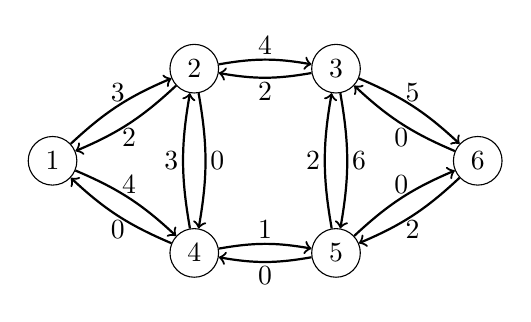
\begin{tikzpicture}[scale=0.9,label distance=-2mm]
        \node[draw, circle] (1) at (1,1.3) {$1$};
        \node[draw, circle] (2) at (3,2.6) {$2$};
        \node[draw, circle] (3) at (5,2.6) {$3$};
        \node[draw, circle] (4) at (7,1.3) {$6$};
        \node[draw, circle] (5) at (3,0) {$4$};
        \node[draw, circle] (6) at (5,0) {$5$};

        \path[draw,thick,->] (1) edge [bend left=10] node[font=\small,label=3] {} (2);
        \path[draw,thick,->] (2) edge [bend left=10] node[font=\small,label=below:2] {} (1);
        \path[draw,thick,->] (2) edge [bend left=10] node[font=\small,label=4] {} (3);
        \path[draw,thick,->] (3) edge [bend left=10] node[font=\small,label=below:2] {} (2);
        \path[draw,thick,->] (3) edge [bend left=10] node[font=\small,label=5] {} (4);
        \path[draw,thick,->] (4) edge [bend left=10] node[font=\small,label=below:0] {} (3);
        \path[draw,thick,->] (1) edge [bend left=10] node[font=\small,label=4] {} (5);
        \path[draw,thick,->] (5) edge [bend left=10] node[font=\small,label=below:0] {} (1);
        \path[draw,thick,->] (5) edge [bend left=10] node[font=\small,label=1] {} (6);
        \path[draw,thick,->] (6) edge [bend left=10] node[font=\small,label=below:0] {} (5);
        \path[draw,thick,->] (6) edge [bend left=10] node[font=\small,label=0] {} (4);
        \path[draw,thick,->] (4) edge [bend left=10] node[font=\small,label=below:2] {} (6);
        \path[draw,thick,->] (5) edge [bend left=10] node[font=\small,label=left:3] {} (2);
        \path[draw,thick,->] (2) edge [bend left=10] node[font=\small,label=right:0] {} (5);
        \path[draw,thick,->] (3) edge [bend left=10] node[font=\small,label=right:6] {} (6);
        \path[draw,thick,->] (6) edge [bend left=10] node[font=\small,label=left:2] {} (3);
    \end{tikzpicture}
\end{center}

La idea es que aumentar el flujo disminuye la cantidad de flujo que
puede pasar por las aristas en el futuro. Por otro lado, es posible
cancelar flujo más tarde utilizando las aristas inversas del grafo
si resulta que sería beneficiario dirigir el flujo de otra manera.

El algoritmo aumenta el flujo siempre y cuando haya un camino de la
fuente al pozo mediante aristas de peso positivo. En el ejemplo,
nuestro próximo camino puede ser el siguiente:

\begin{center}
    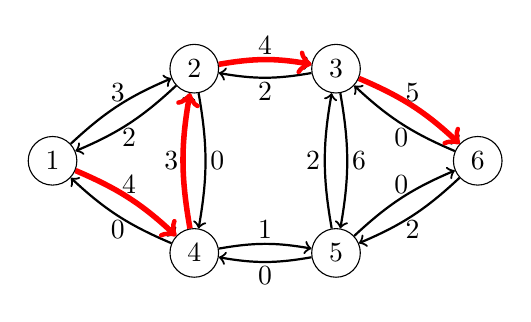
\begin{tikzpicture}[scale=0.9,label distance=-2mm]
        \node[draw, circle] (1) at (1,1.3) {$1$};
        \node[draw, circle] (2) at (3,2.6) {$2$};
        \node[draw, circle] (3) at (5,2.6) {$3$};
        \node[draw, circle] (4) at (7,1.3) {$6$};
        \node[draw, circle] (5) at (3,0) {$4$};
        \node[draw, circle] (6) at (5,0) {$5$};

        \path[draw,thick,->] (1) edge [bend left=10] node[font=\small,label=3] {} (2);
        \path[draw,thick,->] (2) edge [bend left=10] node[font=\small,label=below:2] {} (1);
        \path[draw,thick,->] (2) edge [bend left=10] node[font=\small,label=4] {} (3);
        \path[draw,thick,->] (3) edge [bend left=10] node[font=\small,label=below:2] {} (2);
        \path[draw,thick,->] (3) edge [bend left=10] node[font=\small,label=5] {} (4);
        \path[draw,thick,->] (4) edge [bend left=10] node[font=\small,label=below:0] {} (3);
        \path[draw,thick,->] (1) edge [bend left=10] node[font=\small,label=4] {} (5);
        \path[draw,thick,->] (5) edge [bend left=10] node[font=\small,label=below:0] {} (1);
        \path[draw,thick,->] (5) edge [bend left=10] node[font=\small,label=1] {} (6);
        \path[draw,thick,->] (6) edge [bend left=10] node[font=\small,label=below:0] {} (5);
        \path[draw,thick,->] (6) edge [bend left=10] node[font=\small,label=0] {} (4);
        \path[draw,thick,->] (4) edge [bend left=10] node[font=\small,label=below:2] {} (6);
        \path[draw,thick,->] (5) edge [bend left=10] node[font=\small,label=left:3] {} (2);
        \path[draw,thick,->] (2) edge [bend left=10] node[font=\small,label=right:0] {} (5);
        \path[draw,thick,->] (3) edge [bend left=10] node[font=\small,label=right:6] {} (6);
        \path[draw,thick,->] (6) edge [bend left=10] node[font=\small,label=left:2] {} (3);

        \path[draw=red,thick,->,line width=2pt] (1) edge [bend left=10] (5);
        \path[draw=red,thick,->,line width=2pt] (5) edge [bend left=10] (2);
        \path[draw=red,thick,->,line width=2pt] (2) edge [bend left=10] (3);
        \path[draw=red,thick,->,line width=2pt] (3) edge [bend left=10] (4);
    \end{tikzpicture}
\end{center}

El peso de arista mínimo en este camino es 3, así que el camino aumenta
el flujo por 3, y el flujo total luego de procesar el camino es 5.

El nuevo grafo será de la siguiente manera:

\begin{center}
    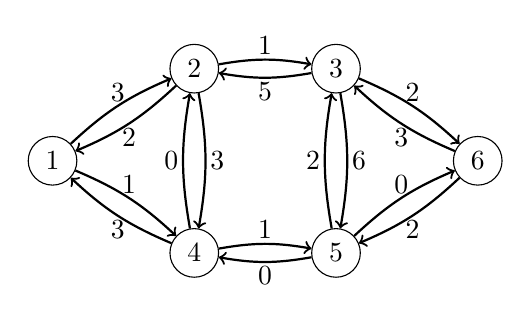
\begin{tikzpicture}[scale=0.9,label distance=-2mm]
        \node[draw, circle] (1) at (1,1.3) {$1$};
        \node[draw, circle] (2) at (3,2.6) {$2$};
        \node[draw, circle] (3) at (5,2.6) {$3$};
        \node[draw, circle] (4) at (7,1.3) {$6$};
        \node[draw, circle] (5) at (3,0) {$4$};
        \node[draw, circle] (6) at (5,0) {$5$};

        \path[draw,thick,->] (1) edge [bend left=10] node[font=\small,label=3] {} (2);
        \path[draw,thick,->] (2) edge [bend left=10] node[font=\small,label=below:2] {} (1);
        \path[draw,thick,->] (2) edge [bend left=10] node[font=\small,label=1] {} (3);
        \path[draw,thick,->] (3) edge [bend left=10] node[font=\small,label=below:5] {} (2);
        \path[draw,thick,->] (3) edge [bend left=10] node[font=\small,label=2] {} (4);
        \path[draw,thick,->] (4) edge [bend left=10] node[font=\small,label=below:3] {} (3);
        \path[draw,thick,->] (1) edge [bend left=10] node[font=\small,label=1] {} (5);
        \path[draw,thick,->] (5) edge [bend left=10] node[font=\small,label=below:3] {} (1);
        \path[draw,thick,->] (5) edge [bend left=10] node[font=\small,label=1] {} (6);
        \path[draw,thick,->] (6) edge [bend left=10] node[font=\small,label=below:0] {} (5);
        \path[draw,thick,->] (6) edge [bend left=10] node[font=\small,label=0] {} (4);
        \path[draw,thick,->] (4) edge [bend left=10] node[font=\small,label=below:2] {} (6);
        \path[draw,thick,->] (5) edge [bend left=10] node[font=\small,label=left:0] {} (2);
        \path[draw,thick,->] (2) edge [bend left=10] node[font=\small,label=right:3] {} (5);
        \path[draw,thick,->] (3) edge [bend left=10] node[font=\small,label=right:6] {} (6);
        \path[draw,thick,->] (6) edge [bend left=10] node[font=\small,label=left:2] {} (3);
    \end{tikzpicture}
\end{center}

Todavía necesitamos dos rondas más antes de alcanzar el flujo máximo.
Por ejemplo, podemos elegir los caminos
$1 \rightarrow 2 \rightarrow 3 \rightarrow 6$ y
$1 \rightarrow 4 \rightarrow 5 \rightarrow 3 \rightarrow 6$.
Ambos aumentan el flujo por 1, y el grafo final es el siguiente:

\begin{center}
    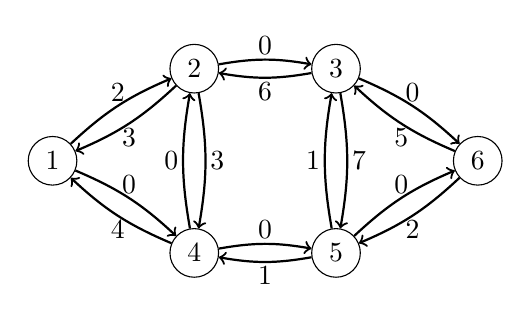
\begin{tikzpicture}[scale=0.9,label distance=-2mm]
        \node[draw, circle] (1) at (1,1.3) {$1$};
        \node[draw, circle] (2) at (3,2.6) {$2$};
        \node[draw, circle] (3) at (5,2.6) {$3$};
        \node[draw, circle] (4) at (7,1.3) {$6$};
        \node[draw, circle] (5) at (3,0) {$4$};
        \node[draw, circle] (6) at (5,0) {$5$};

        \path[draw,thick,->] (1) edge [bend left=10] node[font=\small,label=2] {} (2);
        \path[draw,thick,->] (2) edge [bend left=10] node[font=\small,label=below:3] {} (1);
        \path[draw,thick,->] (2) edge [bend left=10] node[font=\small,label=0] {} (3);
        \path[draw,thick,->] (3) edge [bend left=10] node[font=\small,label=below:6] {} (2);
        \path[draw,thick,->] (3) edge [bend left=10] node[font=\small,label=0] {} (4);
        \path[draw,thick,->] (4) edge [bend left=10] node[font=\small,label=below:5] {} (3);
        \path[draw,thick,->] (1) edge [bend left=10] node[font=\small,label=0] {} (5);
        \path[draw,thick,->] (5) edge [bend left=10] node[font=\small,label=below:4] {} (1);
        \path[draw,thick,->] (5) edge [bend left=10] node[font=\small,label=0] {} (6);
        \path[draw,thick,->] (6) edge [bend left=10] node[font=\small,label=below:1] {} (5);
        \path[draw,thick,->] (6) edge [bend left=10] node[font=\small,label=0] {} (4);
        \path[draw,thick,->] (4) edge [bend left=10] node[font=\small,label=below:2] {} (6);
        \path[draw,thick,->] (5) edge [bend left=10] node[font=\small,label=left:0] {} (2);
        \path[draw,thick,->] (2) edge [bend left=10] node[font=\small,label=right:3] {} (5);
        \path[draw,thick,->] (3) edge [bend left=10] node[font=\small,label=right:7] {} (6);
        \path[draw,thick,->] (6) edge [bend left=10] node[font=\small,label=left:1] {} (3);
    \end{tikzpicture}
\end{center}

No es posible seguir aumentando el flujo, porque no hay un camino
de la fuente al pozo con pesos de arista positivos. Por ende, el
algoritmo termina y el flujo máximo es 7.

\subsubsection{Encontrar caminos}

El algoritmo de Ford--Fulkerson no especifica cómo deberíamos elegir
los caminos que aumenten el flujo. En cualquier caso, el algoritmo
terminará tarde o temprano y encontrará el flujo máximo correctamente.
Sin embargo, la eficiencia del algoritmo depende en la manera en que
elegimos los caminos.

Una forma simple de encontrar caminos es usando una búsqueda en
profundidad. Típicamente esto funciona, pero en el peor caso,
cada camino solo aumentará el flujo por 1 y el algoritmo se vuelve lento.
Afortunadamente, podemos evitar esta situación utilizando una de las
siguientes técnicas:

\index{algoritmo de Edmonds--Karp}

El \key{algoritmo de Edmonds--Karp} \cite{edm72} elige un camino tal
que el número de aristas en el camino sea tan pequeño como sea posible.
Esto se puede hacer con una búsqueda en anchura en vez de una búsqueda
en profundidad para encontrar caminos. Se puede demostrar que esto
garantiza que el flujo aumentará rápidamente, y la complejidad temporal
del algoritmo es $O(m^2 n)$.

\index{algoritmo escalador}

El \key{algoritmo escalador} \cite{ahu91} utiliza una búsqueda en
profundidad para encontrar caminos donde cada peso de arista alcance
un valor umbral. Inicialmente, el valor umbral es un número
grande---por ejemplo la suma de todos los pesos en el grafo. Siempre
que un camino no se pueda encontrar, el umbral es dividido por 2. La
complejidad del algoritmo es $O(m^2 \log c)$, donde $c$ es el valor
de umbral inicial.

En la práctica, el algoritmo escalador es más fácil de implementar,
porque se puede utilizar la búsqueda en profundidad para encontrar
caminos. Ambos algoritmos son suficientemente eficientes para
los problemas típicos de programación competitiva.

\subsubsection{Corte mínimo}

\index{corte mínimo}

Resulta que una vez que el algoritmo de Ford--Fulkerson ha encontrado
un flujo máximo, también ha determinado un corte mínimo. Definamos
$A$ como el conjunto de nodos alcanzables desde la fuente utilizando
aristas de peso positivo. En el grafo de ejemplo, $A$ contiene los nodos
1, 2, y 4:

\begin{center}
    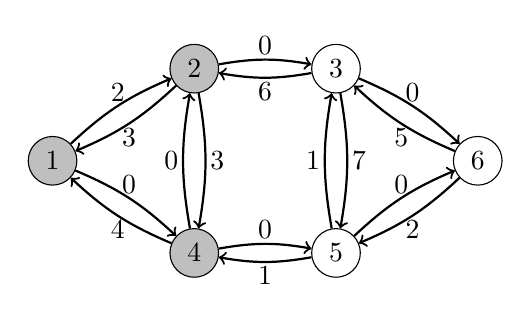
\begin{tikzpicture}[scale=0.9,label distance=-2mm]
        \node[draw, circle,fill=lightgray] (1) at (1,1.3) {$1$};
        \node[draw, circle,fill=lightgray] (2) at (3,2.6) {$2$};
        \node[draw, circle] (3) at (5,2.6) {$3$};
        \node[draw, circle] (4) at (7,1.3) {$6$};
        \node[draw, circle,fill=lightgray] (5) at (3,0) {$4$};
        \node[draw, circle] (6) at (5,0) {$5$};

        \path[draw,thick,->] (1) edge [bend left=10] node[font=\small,label=2] {} (2);
        \path[draw,thick,->] (2) edge [bend left=10] node[font=\small,label=below:3] {} (1);
        \path[draw,thick,->] (2) edge [bend left=10] node[font=\small,label=0] {} (3);
        \path[draw,thick,->] (3) edge [bend left=10] node[font=\small,label=below:6] {} (2);
        \path[draw,thick,->] (3) edge [bend left=10] node[font=\small,label=0] {} (4);
        \path[draw,thick,->] (4) edge [bend left=10] node[font=\small,label=below:5] {} (3);
        \path[draw,thick,->] (1) edge [bend left=10] node[font=\small,label=0] {} (5);
        \path[draw,thick,->] (5) edge [bend left=10] node[font=\small,label=below:4] {} (1);
        \path[draw,thick,->] (5) edge [bend left=10] node[font=\small,label=0] {} (6);
        \path[draw,thick,->] (6) edge [bend left=10] node[font=\small,label=below:1] {} (5);
        \path[draw,thick,->] (6) edge [bend left=10] node[font=\small,label=0] {} (4);
        \path[draw,thick,->] (4) edge [bend left=10] node[font=\small,label=below:2] {} (6);
        \path[draw,thick,->] (5) edge [bend left=10] node[font=\small,label=left:0] {} (2);
        \path[draw,thick,->] (2) edge [bend left=10] node[font=\small,label=right:3] {} (5);
        \path[draw,thick,->] (3) edge [bend left=10] node[font=\small,label=right:7] {} (6);
        \path[draw,thick,->] (6) edge [bend left=10] node[font=\small,label=left:1] {} (3);
    \end{tikzpicture}
\end{center}

Ahora el corte mínimo consiste de las aristas del grafo original
que comienzan en algún nodo en $A$, terminan en algún nodo fuera de $A$,
y cuyas capacidades son enteramente utilizadas en el flujo máximo. En el
grafo de arriba, tales aristas son $2 \rightarrow 3$ y
$4 \rightarrow 5$, que corresponden al corte mínimo $6+1=7$.

¿Por qué el flujo producido por el algoritmo es máximo, y el
corte es mínimo? La razón es que el grafo no puede contener un flujo
cuyo tamaño sea mayor que el peso de cualquier corte del grafo. Por ende,
siempre que un flujo y un corte sean iguales, son un flujo máximo y
un corte mínimo.

Consideremos cualquier corte del grafo tal que la fuente pertenezca
a $A$, el pozo pertenezca a $B$, y haya algunas aristas entre los
conjuntos:

\begin{center}
    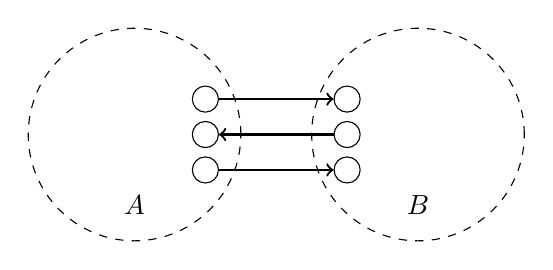
\begin{tikzpicture}[scale=0.9]
        \draw[dashed] (-2,0) circle (1.5);
        \draw[dashed] (2,0) circle (1.5);

        \node at (-2,-1) {$A$};
        \node at (2,-1) {$B$};

        \node[draw, circle] (1) at (-1,0.5) {};
        \node[draw, circle] (2) at (-1,0) {};
        \node[draw, circle] (3) at (-1,-0.5) {};
        \node[draw, circle] (4) at (1,0.5) {};
        \node[draw, circle] (5) at (1,0) {};
        \node[draw, circle] (6) at (1,-0.5) {};

        \path[draw,thick,->] (1) -- (4);
        \path[draw,thick,->] (5) -- (2);
        \path[draw,thick,->] (3) -- (6);

    \end{tikzpicture}
\end{center}

El tamaño del corte es la suma de las aristas que van de $A$ a $B$.
Este es un límite inferior para el flujo en el grafo, porque el flujo
debe proceder de $A$ a $B$. Por lo tanto, el tamaño del flujo máximo
es menor o igual a aquel de cualquier corte en el grafo.

Por otro lado, el algoritmo de Ford--Fulkerson produce un flujo
cuyo tamaño es \emph{exactamente} igual al de algún corte en el grafo.
Por esto, el flujo debe ser un flujo máximo y el corte debe ser mínimo.

\section{Caminos disjuntos}

Muchos problemas de grafos pueden ser resueltos si los reducimos al
problema de flujo máximo. Nuestro primer ejemplo de tal problema es el
siguiente: recibimos un grafo dirigido con una fuente y un pozo, y
nuestra tarea es encontrar el máximo número de caminos disjuntos desde
la fuente hasta el pozo.

\subsubsection{Caminos disjuntos en aristas}

Primero nos centraremos en el problema de encontrar el máximo número
de \key{caminos disjuntos en aristas} de la fuente al pozo. Esto
significa que debemos construir un conjunto de caminos tal que cada
arista aparezca como mucho en un camino.

Por ejemplo, veamos el siguiente grafo:
\begin{center}
    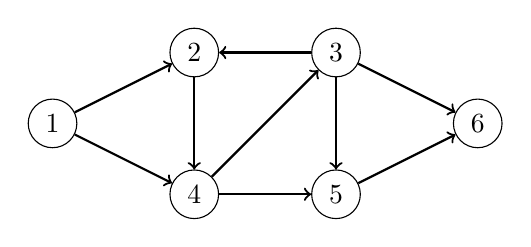
\begin{tikzpicture}[scale=0.9]
        \node[draw, circle] (1) at (1,2) {$1$};
        \node[draw, circle] (2) at (3,3) {$2$};
        \node[draw, circle] (3) at (5,3) {$3$};
        \node[draw, circle] (4) at (3,1) {$4$};
        \node[draw, circle] (5) at (5,1) {$5$};
        \node[draw, circle] (6) at (7,2) {$6$};
        \path[draw,thick,->] (1) -- (2);
        \path[draw,thick,->] (1) -- (4);
        \path[draw,thick,->] (2) -- (4);
        \path[draw,thick,->] (3) -- (2);
        \path[draw,thick,->] (3) -- (5);
        \path[draw,thick,->] (3) -- (6);
        \path[draw,thick,->] (4) -- (3);
        \path[draw,thick,->] (4) -- (5);
        \path[draw,thick,->] (5) -- (6);
    \end{tikzpicture}
\end{center}

En este grafo, el máximo número de caminos disjuntos en aristas es 2.
Podemos elegir los caminos
$1 \rightarrow 2 \rightarrow 4 \rightarrow 3 \rightarrow 6$
y $1 \rightarrow 4 \rightarrow 5 \rightarrow 6$ como sigue:

\begin{center}
    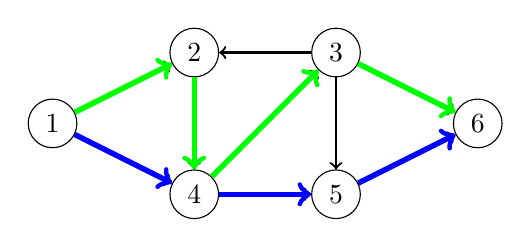
\begin{tikzpicture}[scale=0.9]
        \node[draw, circle] (1) at (1,2) {$1$};
        \node[draw, circle] (2) at (3,3) {$2$};
        \node[draw, circle] (3) at (5,3) {$3$};
        \node[draw, circle] (4) at (3,1) {$4$};
        \node[draw, circle] (5) at (5,1) {$5$};
        \node[draw, circle] (6) at (7,2) {$6$};
        \path[draw,thick,->] (1) -- (2);
        \path[draw,thick,->] (1) -- (4);
        \path[draw,thick,->] (2) -- (4);
        \path[draw,thick,->] (3) -- (2);
        \path[draw,thick,->] (3) -- (5);
        \path[draw,thick,->] (3) -- (6);
        \path[draw,thick,->] (4) -- (3);
        \path[draw,thick,->] (4) -- (5);
        \path[draw,thick,->] (5) -- (6);

        \path[draw=green,thick,->,line width=2pt] (1) -- (2);
        \path[draw=green,thick,->,line width=2pt] (2) -- (4);
        \path[draw=green,thick,->,line width=2pt] (4) -- (3);
        \path[draw=green,thick,->,line width=2pt] (3) -- (6);

        \path[draw=blue,thick,->,line width=2pt] (1) -- (4);
        \path[draw=blue,thick,->,line width=2pt] (4) -- (5);
        \path[draw=blue,thick,->,line width=2pt] (5) -- (6);
    \end{tikzpicture}
\end{center}

Resulta que el máximo número de caminos disjuntos en aristas es igual
al máximo flujo del grafo, asumiendo que la capacidad de cada arista
es 1. Una vez que el máximo flujo ha sido construido, los caminos
disjuntos en aristas pueden encontrarse vorazmente siguiendo caminos de
la fuente al pozo.

\subsubsection{Caminos disjuntos en nodos}

Ahora considera otro problema: encontrar el máximo número de
\key{caminos disjuntos en nodos} de la fuente al pozo. En este problema,
cada nodo, excepto por la fuente y el pozo, puede aparecer como mucho
en un camino. El número de caminos disjuntos en nodos puede ser
menor que el de caminos disjuntos en aristas. Por ejemplo, en el
grafo previo, el máximo número de caminos disjuntos en nodos es 1:

\begin{center}
    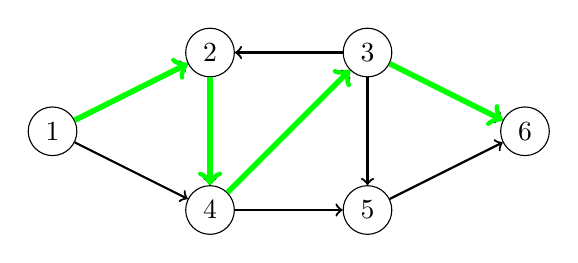
\begin{tikzpicture}
        \node[draw, circle] (1) at (1,2) {$1$};
        \node[draw, circle] (2) at (3,3) {$2$};
        \node[draw, circle] (3) at (5,3) {$3$};
        \node[draw, circle] (4) at (3,1) {$4$};
        \node[draw, circle] (5) at (5,1) {$5$};
        \node[draw, circle] (6) at (7,2) {$6$};
        \path[draw,thick,->] (1) -- (2);
        \path[draw,thick,->] (1) -- (4);
        \path[draw,thick,->] (2) -- (4);
        \path[draw,thick,->] (3) -- (2);
        \path[draw,thick,->] (3) -- (5);
        \path[draw,thick,->] (3) -- (6);
        \path[draw,thick,->] (4) -- (3);
        \path[draw,thick,->] (4) -- (5);
        \path[draw,thick,->] (5) -- (6);

        \path[draw=green,thick,->,line width=2pt] (1) -- (2);
        \path[draw=green,thick,->,line width=2pt] (2) -- (4);
        \path[draw=green,thick,->,line width=2pt] (4) -- (3);
        \path[draw=green,thick,->,line width=2pt] (3) -- (6);
    \end{tikzpicture}
\end{center}

Podemos reducir este problema al problema del máximo flujo. Ya que
cada nodo puede aparecer en un camino como mucho, debemos limitar el
flujo que pasa por los nodos. Un método estándar para hacer esto es
dividir cada nodo en dos nodos tal que el primero tenga las aristas
de entrada del nodo original, el segundo las aristas de salida del
nodo original, y haya una nueva arista del primer nodo al segundo.

En nuestro ejemplo, el grafo se convierte en el siguiente:
\begin{center}
    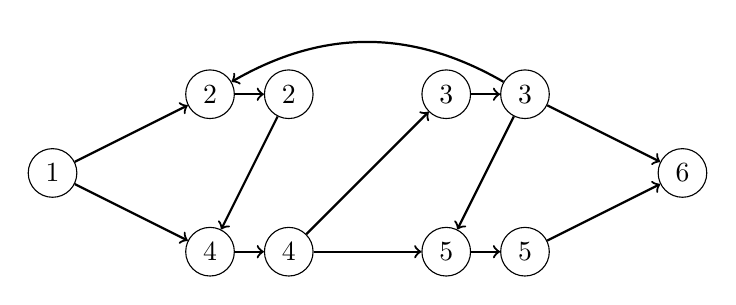
\begin{tikzpicture}
        \node[draw, circle] (1) at (1,2) {$1$};

        \node[draw, circle] (2a) at (3,3) {$2$};
        \node[draw, circle] (3a) at (6,3) {$3$};
        \node[draw, circle] (4a) at (3,1) {$4$};
        \node[draw, circle] (5a) at (6,1) {$5$};

        \node[draw, circle] (2b) at (4,3) {$2$};
        \node[draw, circle] (3b) at (7,3) {$3$};
        \node[draw, circle] (4b) at (4,1) {$4$};
        \node[draw, circle] (5b) at (7,1) {$5$};

        \node[draw, circle] (6) at (9,2) {$6$};

        \path[draw,thick,->] (2a) -- (2b);
        \path[draw,thick,->] (3a) -- (3b);
        \path[draw,thick,->] (4a) -- (4b);
        \path[draw,thick,->] (5a) -- (5b);

        \path[draw,thick,->] (1) -- (2a);
        \path[draw,thick,->] (1) -- (4a);
        \path[draw,thick,->] (2b) -- (4a);
        \path[draw,thick,->] (3b) edge [bend right=30] (2a);
        \path[draw,thick,->] (3b) -- (5a);
        \path[draw,thick,->] (3b) -- (6);
        \path[draw,thick,->] (4b) -- (3a);
        \path[draw,thick,->] (4b) -- (5a);
        \path[draw,thick,->] (5b) -- (6);
    \end{tikzpicture}
\end{center}

El flujo máximo para el grafo es el siguiente:
\begin{center}
    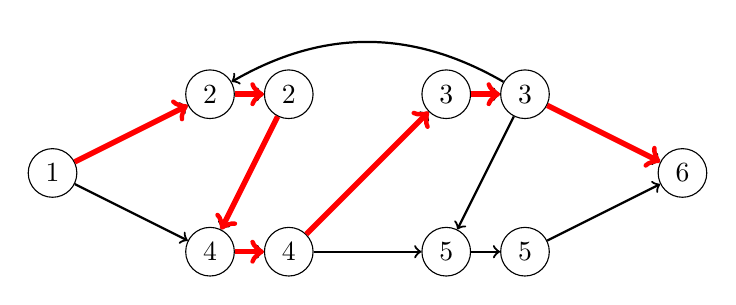
\begin{tikzpicture}
        \node[draw, circle] (1) at (1,2) {$1$};

        \node[draw, circle] (2a) at (3,3) {$2$};
        \node[draw, circle] (3a) at (6,3) {$3$};
        \node[draw, circle] (4a) at (3,1) {$4$};
        \node[draw, circle] (5a) at (6,1) {$5$};

        \node[draw, circle] (2b) at (4,3) {$2$};
        \node[draw, circle] (3b) at (7,3) {$3$};
        \node[draw, circle] (4b) at (4,1) {$4$};
        \node[draw, circle] (5b) at (7,1) {$5$};

        \node[draw, circle] (6) at (9,2) {$6$};

        \path[draw,thick,->] (2a) -- (2b);
        \path[draw,thick,->] (3a) -- (3b);
        \path[draw,thick,->] (4a) -- (4b);
        \path[draw,thick,->] (5a) -- (5b);

        \path[draw,thick,->] (1) -- (2a);
        \path[draw,thick,->] (1) -- (4a);
        \path[draw,thick,->] (2b) -- (4a);
        \path[draw,thick,->] (3b) edge [bend right=30] (2a);
        \path[draw,thick,->] (3b) -- (5a);
        \path[draw,thick,->] (3b) -- (6);
        \path[draw,thick,->] (4b) -- (3a);
        \path[draw,thick,->] (4b) -- (5a);
        \path[draw,thick,->] (5b) -- (6);

        \path[draw=red,thick,->,line width=2pt] (1) -- (2a);
        \path[draw=red,thick,->,line width=2pt] (2a) -- (2b);
        \path[draw=red,thick,->,line width=2pt] (2b) -- (4a);
        \path[draw=red,thick,->,line width=2pt] (4a) -- (4b);
        \path[draw=red,thick,->,line width=2pt] (4b) -- (3a);
        \path[draw=red,thick,->,line width=2pt] (3a) -- (3b);
        \path[draw=red,thick,->,line width=2pt] (3b) -- (6);
    \end{tikzpicture}
\end{center}

Por ende, el máximo número de caminos disjuntos en nodos de la fuente
al pozo es 1.

\section{\textit{Matchings} máximos}

\index{matchings máximos@\textit{matchings} máximos}

El problema de \key{\textit{matchings} máximos} nos pide encontrar
un conjunto de tamaño máximo de pares de nodos en un grafo no dirigido
tal que cada par esté conectado con una arista y cada nodo pertenezca
a lo sumo a un par de nodos.

Existen algoritmos polinomiales para encontrar matchings máximos en
grafos generales \cite{edm65}, pero tales algoritmos son complejos
y raramente vistos en competiciones de programación. Sin embargo, en
grafos bipartitos, el problema de encontrar matchings máximos es mucho
más fácil de resolver, porque podemos reducirlo al problema de flujo
máximo.

\subsubsection{Encontrar \textit{matchings} máximos}

Los nodos de un grafo bipartito siempre pueden dividirse en dos grupos
tal que todas las aristas del grafo vayan del grupo izquierdo al grupo
derecho. Por ejemplo, en el siguiente grafo bipartito, los grupos
son $\{1,2,3,4\}$ y $\{5,6,7,8\}$.

\begin{center}
    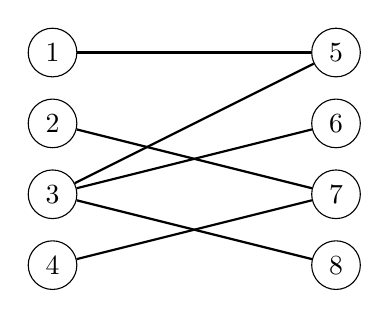
\begin{tikzpicture}[scale=0.60]
        \node[draw, circle] (1) at (2,4.5) {1};
        \node[draw, circle] (2) at (2,3) {2};
        \node[draw, circle] (3) at (2,1.5) {3};
        \node[draw, circle] (4) at (2,0) {4};
        \node[draw, circle] (5) at (8,4.5) {5};
        \node[draw, circle] (6) at (8,3) {6};
        \node[draw, circle] (7) at (8,1.5) {7};
        \node[draw, circle] (8) at (8,0) {8};

        \path[draw,thick,-] (1) -- (5);
        \path[draw,thick,-] (2) -- (7);
        \path[draw,thick,-] (3) -- (5);
        \path[draw,thick,-] (3) -- (6);
        \path[draw,thick,-] (3) -- (8);
        \path[draw,thick,-] (4) -- (7);
    \end{tikzpicture}
\end{center}
El tamaño de un matching máximo en este grafo es 3:
\begin{center}
    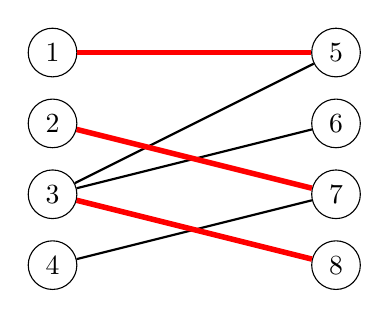
\begin{tikzpicture}[scale=0.60]
        \node[draw, circle] (1) at (2,4.5) {1};
        \node[draw, circle] (2) at (2,3) {2};
        \node[draw, circle] (3) at (2,1.5) {3};
        \node[draw, circle] (4) at (2,0) {4};
        \node[draw, circle] (5) at (8,4.5) {5};
        \node[draw, circle] (6) at (8,3) {6};
        \node[draw, circle] (7) at (8,1.5) {7};
        \node[draw, circle] (8) at (8,0) {8};

        \path[draw,thick,-] (1) -- (5);
        \path[draw,thick,-] (2) -- (7);
        \path[draw,thick,-] (3) -- (5);
        \path[draw,thick,-] (3) -- (6);
        \path[draw,thick,-] (3) -- (8);
        \path[draw,thick,-] (4) -- (7);

        \path[draw=red,thick,-,line width=2pt] (1) -- (5);
        \path[draw=red,thick,-,line width=2pt] (2) -- (7);
        \path[draw=red,thick,-,line width=2pt] (3) -- (8);
    \end{tikzpicture}
\end{center}

Podemos reducir el problema del matching máximo bipartito al problema
del flujo máximo si añadimos dos nuevos nodos al grafo: una fuente y
un pozo. También añadimos aristas de la fuente a cada nodo izquierdo y
de cada nodo derecho al pozo. Luego de esto, el tamaño de un flujo
máximo en el grafo equivale al tamaño de un matching máximo en el grafo
original.

Por ejemplo, la reducción para el grafo de arriba es la siguiente:
\begin{center}
    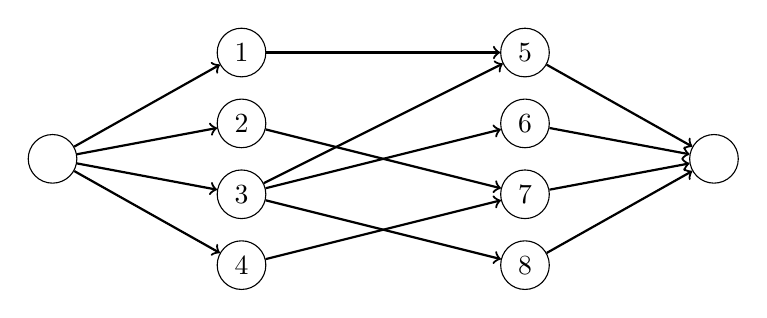
\begin{tikzpicture}[scale=0.60]
        \node[draw, circle] (1) at (2,4.5) {1};
        \node[draw, circle] (2) at (2,3) {2};
        \node[draw, circle] (3) at (2,1.5) {3};
        \node[draw, circle] (4) at (2,0) {4};
        \node[draw, circle] (5) at (8,4.5) {5};
        \node[draw, circle] (6) at (8,3) {6};
        \node[draw, circle] (7) at (8,1.5) {7};
        \node[draw, circle] (8) at (8,0) {8};

        \node[draw, circle] (a) at (-2,2.25) {\phantom{0}};
        \node[draw, circle] (b) at (12,2.25) {\phantom{0}};

        \path[draw,thick,->] (1) -- (5);
        \path[draw,thick,->] (2) -- (7);
        \path[draw,thick,->] (3) -- (5);
        \path[draw,thick,->] (3) -- (6);
        \path[draw,thick,->] (3) -- (8);
        \path[draw,thick,->] (4) -- (7);

        \path[draw,thick,->] (a) -- (1);
        \path[draw,thick,->] (a) -- (2);
        \path[draw,thick,->] (a) -- (3);
        \path[draw,thick,->] (a) -- (4);
        \path[draw,thick,->] (5) -- (b);
        \path[draw,thick,->] (6) -- (b);
        \path[draw,thick,->] (7) -- (b);
        \path[draw,thick,->] (8) -- (b);
    \end{tikzpicture}
\end{center}

El flujo máximo de este grafo es el siguiente:
\begin{center}
    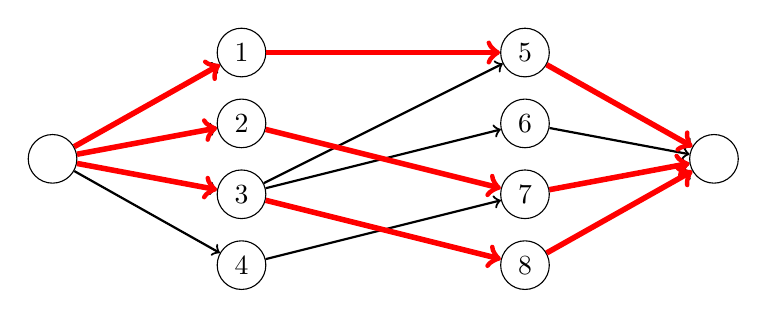
\begin{tikzpicture}[scale=0.60]
        \node[draw, circle] (1) at (2,4.5) {1};
        \node[draw, circle] (2) at (2,3) {2};
        \node[draw, circle] (3) at (2,1.5) {3};
        \node[draw, circle] (4) at (2,0) {4};
        \node[draw, circle] (5) at (8,4.5) {5};
        \node[draw, circle] (6) at (8,3) {6};
        \node[draw, circle] (7) at (8,1.5) {7};
        \node[draw, circle] (8) at (8,0) {8};

        \node[draw, circle] (a) at (-2,2.25) {\phantom{0}};
        \node[draw, circle] (b) at (12,2.25) {\phantom{0}};

        \path[draw,thick,->] (3) -- (5);
        \path[draw,thick,->] (3) -- (6);
        \path[draw,thick,->] (4) -- (7);

        \path[draw,thick,->] (a) -- (1);
        \path[draw,thick,->] (a) -- (2);
        \path[draw,thick,->] (a) -- (3);
        \path[draw,thick,->] (a) -- (4);
        \path[draw,thick,->] (5) -- (b);
        \path[draw,thick,->] (6) -- (b);
        \path[draw,thick,->] (7) -- (b);
        \path[draw,thick,->] (8) -- (b);

        \path[draw=red,thick,->,line width=2pt] (1) -- (5);
        \path[draw=red,thick,->,line width=2pt] (2) -- (7);
        \path[draw=red,thick,->,line width=2pt] (3) -- (8);

        \path[draw=red,thick,->,line width=2pt] (a) -- (1);
        \path[draw=red,thick,->,line width=2pt] (a) -- (2);
        \path[draw=red,thick,->,line width=2pt] (a) -- (3);

        \path[draw=red,thick,->,line width=2pt] (5) -- (b);
        \path[draw=red,thick,->,line width=2pt] (7) -- (b);
        \path[draw=red,thick,->,line width=2pt] (8) -- (b);

    \end{tikzpicture}
\end{center}

\subsubsection{Teorema de Hall}

\index{teorema de Hall}
\index{matching perfecto@\textit{matching} perfecto}

El \key{teorema de Hall} puede utilizarse para encontrar si un grafo
bipartito tiene un matching que contenga todos los nodos izquierdos o
derechos. Si el número de nodos izquierdos y derechos es el mismo, el
teorema nos dice si es posible construir un \key{matching perfecto}---un
matching que contenga todos los nodos del grafo.

Asume que queremos encontrar un matching que contenga todos los nodos
izquierdos. Definamos $X$ como cualquier conjunto de nodos izquierdos
y $f(X)$ como el conjunto de sus vecinos. Según el teorema de Hall, un
matching que contiene todos los nodos izquierdos existe exactamente
cuando por cada $X$, la condición $|X| \le |f(x)|$ es verdadera.

Estudiemos el teorema de Hall en el grafo de ejemplo. Primero,
definamos $X=\{1,3\}$ que resulta en $f(X)=\{5,6,8\}$:

\begin{center}
    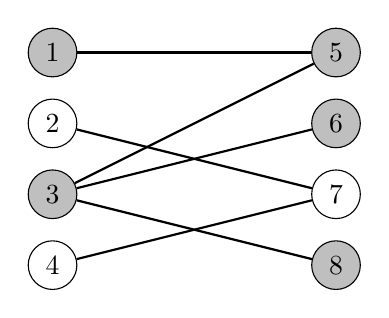
\begin{tikzpicture}[scale=0.60]
        \node[draw, circle, fill=lightgray] (1) at (2,4.5) {1};
        \node[draw, circle] (2) at (2,3) {2};
        \node[draw, circle, fill=lightgray] (3) at (2,1.5) {3};
        \node[draw, circle] (4) at (2,0) {4};
        \node[draw, circle, fill=lightgray] (5) at (8,4.5) {5};
        \node[draw, circle, fill=lightgray] (6) at (8,3) {6};
        \node[draw, circle] (7) at (8,1.5) {7};
        \node[draw, circle, fill=lightgray] (8) at (8,0) {8};

        \path[draw,thick,-] (1) -- (5);
        \path[draw,thick,-] (2) -- (7);
        \path[draw,thick,-] (3) -- (5);
        \path[draw,thick,-] (3) -- (6);
        \path[draw,thick,-] (3) -- (8);
        \path[draw,thick,-] (4) -- (7);
    \end{tikzpicture}
\end{center}

La condición del teorema de Hall se cumple, porque $|X|=2$ y $|f(X)|=3$.
Ahora, definamos $X=\{2,4\}$ que resuta en $f(X)=\{7\}$:

\begin{center}
    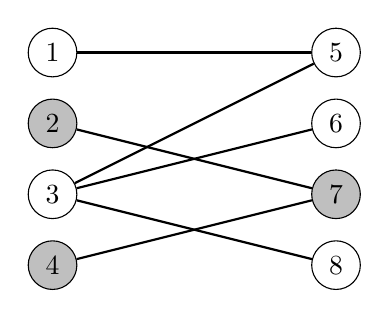
\begin{tikzpicture}[scale=0.60]
        \node[draw, circle] (1) at (2,4.5) {1};
        \node[draw, circle, fill=lightgray] (2) at (2,3) {2};
        \node[draw, circle] (3) at (2,1.5) {3};
        \node[draw, circle, fill=lightgray] (4) at (2,0) {4};
        \node[draw, circle] (5) at (8,4.5) {5};
        \node[draw, circle] (6) at (8,3) {6};
        \node[draw, circle, fill=lightgray] (7) at (8,1.5) {7};
        \node[draw, circle] (8) at (8,0) {8};

        \path[draw,thick,-] (1) -- (5);
        \path[draw,thick,-] (2) -- (7);
        \path[draw,thick,-] (3) -- (5);
        \path[draw,thick,-] (3) -- (6);
        \path[draw,thick,-] (3) -- (8);
        \path[draw,thick,-] (4) -- (7);
    \end{tikzpicture}
\end{center}

En este caso, $|X|=2$ y $|f(X)|=1$, así que la condición del teorema
de Hall no se cumple. Esto significa que no es posible formar un
matching perfecto para este grafo. El resultado no es sorprendente,
porque ya sabemos que el matching máximo del grafo es 3 y no 4.

Si la condición del teorema de Hall no se cumple, el conjunto $X$
provee una explicación de \emph{por qué} no podemos formar tal matching.
Debido a que $X$ contiene más nodos que $f(X)$, no hay pares para todos
los nodos en $X$. Por ejemplo, en el grafo de arriba, los dos nodos 2 y
4 deberían estar conectados con el nodo 7, que es imposible.

\subsubsection{Teorema de Kőnig}

\index{teorema de Kőnig}
\index{cobertura de nodos mínima}

Una \key{cobertura de nodos mínima} de un grafo es un mínimo conjunto
de nodos tal que cada arista del grafo tenga por lo menos un extremo
en el conjunto. En un grafo general, encontrar una cobertura de nodos
mínima es un problema NP-difícil. No obstante, si el grafo es bipartito,
el \key{teorema de Kőnig} nos dice que el tamaño de una cobertura de
nodos mínima y el tamaño de un matching máximo siempre son iguales.
Por lo tanto, podemos calcular el tamaño de la cobertura de nodos mínima
utilizando un algoritmo de flujo máximo.

Considera el siguiente grafo con un matching máximo de tamaño 3:
\begin{center}
    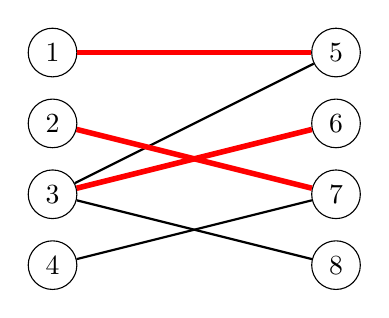
\begin{tikzpicture}[scale=0.60]
        \node[draw, circle] (1) at (2,4.5) {1};
        \node[draw, circle] (2) at (2,3) {2};
        \node[draw, circle] (3) at (2,1.5) {3};
        \node[draw, circle] (4) at (2,0) {4};
        \node[draw, circle] (5) at (8,4.5) {5};
        \node[draw, circle] (6) at (8,3) {6};
        \node[draw, circle] (7) at (8,1.5) {7};
        \node[draw, circle] (8) at (8,0) {8};

        \path[draw,thick,-] (1) -- (5);
        \path[draw,thick,-] (2) -- (7);
        \path[draw,thick,-] (3) -- (5);
        \path[draw,thick,-] (3) -- (6);
        \path[draw,thick,-] (3) -- (8);
        \path[draw,thick,-] (4) -- (7);

        \path[draw=red,thick,-,line width=2pt] (1) -- (5);
        \path[draw=red,thick,-,line width=2pt] (2) -- (7);
        \path[draw=red,thick,-,line width=2pt] (3) -- (6);
    \end{tikzpicture}
\end{center}
Ahora el teorema de Kőnig nos dice que el tamaño de la cobertura de
nodos mínima es también 3. Una cobertura tal puede construirse así:
\begin{center}
    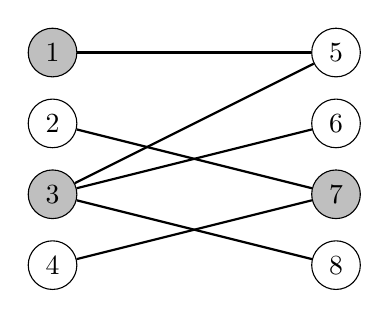
\begin{tikzpicture}[scale=0.60]
        \node[draw, circle, fill=lightgray] (1) at (2,4.5) {1};
        \node[draw, circle] (2) at (2,3) {2};
        \node[draw, circle, fill=lightgray] (3) at (2,1.5) {3};
        \node[draw, circle] (4) at (2,0) {4};
        \node[draw, circle] (5) at (8,4.5) {5};
        \node[draw, circle] (6) at (8,3) {6};
        \node[draw, circle, fill=lightgray] (7) at (8,1.5) {7};
        \node[draw, circle] (8) at (8,0) {8};

        \path[draw,thick,-] (1) -- (5);
        \path[draw,thick,-] (2) -- (7);
        \path[draw,thick,-] (3) -- (5);
        \path[draw,thick,-] (3) -- (6);
        \path[draw,thick,-] (3) -- (8);
        \path[draw,thick,-] (4) -- (7);
    \end{tikzpicture}
\end{center}

\index{conjunto independiente máximo}

Los nodos que \emph{no} pertenecen a una cobertura de nodos mínima
forman un \key{conjunto independiente máximo}. Este es el conjunto de
nodos más grande tal que no haya algún par de nodos en el conjunto
conectado por una arista. Nuevamente, encontrar el conjunto
independiente en un grafo general es un problema NP-difícil, pero en
un grafo bipartito podemos usar el teorema de Kőnig para resolver el
problema eficientemente. En el grafo de ejemplo, el conjunto
independiente máximo es el siguiente:

\begin{center}
    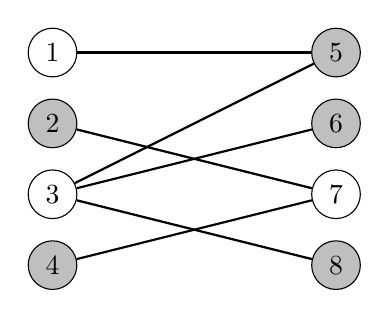
\begin{tikzpicture}[scale=0.60]
        \node[draw, circle] (1) at (2,4.5) {1};
        \node[draw, circle, fill=lightgray] (2) at (2,3) {2};
        \node[draw, circle] (3) at (2,1.5) {3};
        \node[draw, circle, fill=lightgray] (4) at (2,0) {4};
        \node[draw, circle, fill=lightgray] (5) at (8,4.5) {5};
        \node[draw, circle, fill=lightgray] (6) at (8,3) {6};
        \node[draw, circle] (7) at (8,1.5) {7};
        \node[draw, circle, fill=lightgray] (8) at (8,0) {8};

        \path[draw,thick,-] (1) -- (5);
        \path[draw,thick,-] (2) -- (7);
        \path[draw,thick,-] (3) -- (5);
        \path[draw,thick,-] (3) -- (6);
        \path[draw,thick,-] (3) -- (8);
        \path[draw,thick,-] (4) -- (7);
    \end{tikzpicture}
\end{center}

\section{Cobertura de caminos}

\index{cobertura de caminos}

Una \key{cobertura de caminos} es un conjunto de caminos de un grafo
tal que cada nodo del grafo pertenezca a por lo menos un camino.
Resulta que en un grafo acíclico dirigido, podemos reducir este problema
al de encontrar el flujo máximo en otro grafo.

\subsubsection{Cobertura de caminos disjunta en nodos}

En una \key{cobertura de caminos disjunta en nodos}, cada nodo pertenece
a exactamente un camino. Por ejemplo, considera el siguiente grafo:
\begin{center}
    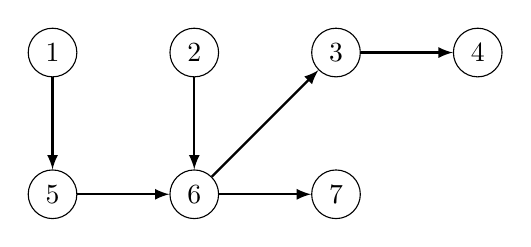
\begin{tikzpicture}[scale=0.9]
        \node[draw, circle] (1) at (0,0) {1};
        \node[draw, circle] (2) at (2,0) {2};
        \node[draw, circle] (3) at (4,0) {3};
        \node[draw, circle] (4) at (6,0) {4};
        \node[draw, circle] (5) at (0,-2) {5};
        \node[draw, circle] (6) at (2,-2) {6};
        \node[draw, circle] (7) at (4,-2) {7};

        \path[draw,thick,->,>=latex] (1) -- (5);
        \path[draw,thick,->,>=latex] (2) -- (6);
        \path[draw,thick,->,>=latex] (3) -- (4);
        \path[draw,thick,->,>=latex] (5) -- (6);
        \path[draw,thick,->,>=latex] (6) -- (3);
        \path[draw,thick,->,>=latex] (6) -- (7);
    \end{tikzpicture}
\end{center}

Una mínima cobertura de caminos disjunta en nodos de este grafo
consiste de tres caminos. Por ejemplo, podemos elegir los siguientes:

\begin{center}
    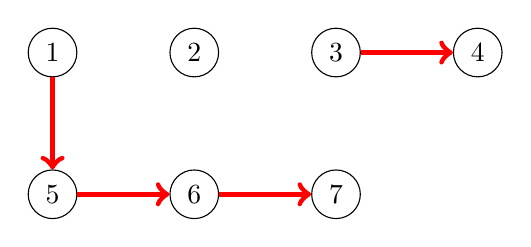
\begin{tikzpicture}[scale=0.9]
        \node[draw, circle] (1) at (0,0) {1};
        \node[draw, circle] (2) at (2,0) {2};
        \node[draw, circle] (3) at (4,0) {3};
        \node[draw, circle] (4) at (6,0) {4};
        \node[draw, circle] (5) at (0,-2) {5};
        \node[draw, circle] (6) at (2,-2) {6};
        \node[draw, circle] (7) at (4,-2) {7};

        \path[draw=red,thick,->,line width=2pt] (1) -- (5);
        \path[draw=red,thick,->,line width=2pt] (5) -- (6);
        \path[draw=red,thick,->,line width=2pt] (6) -- (7);
        \path[draw=red,thick,->,line width=2pt] (3) -- (4);
    \end{tikzpicture}
\end{center}

Ten en cuenta que uno de los caminos solo contiene el nodo 2,
así que no es posible que un camino no contenga ninguna arista.

Podemos encontrar una cobertura de caminos disjunta en nodos
construyendo un \emph{grafo de matchings} donde cada nodo del grafo
original esté representado por dos nodos: uno izquierdo y uno derecho.
Hay una arista de un nodo izquierdo a un nodo derecho si hay tal arista
en el grafo original. Adicionalmente, el grafo de matchings contiene
una fuente y un pozo, y hay aristas de la fuente a todos los nodos
izquierdos y de todos los nodos derechos al pozo.

Un matching máximo en el grafo resultante corresponde a una mínima
cobertura de caminos disjunta en nodos en el grafo original. Por ejemplo,
el siguiente grafo de matchings para el grafo de arriba contiene un
matching máximo de 4:

\begin{center}
    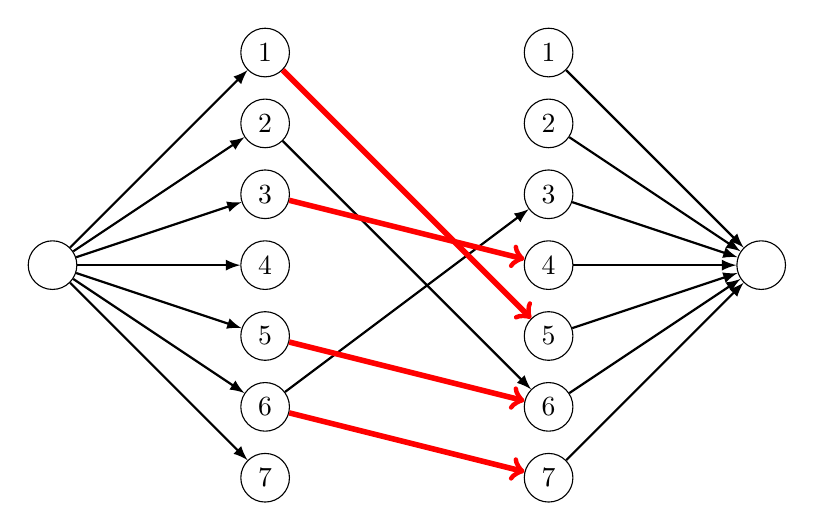
\begin{tikzpicture}[scale=0.9]
        \node[draw, circle] (1a) at (0,6) {1};
        \node[draw, circle] (2a) at (0,5) {2};
        \node[draw, circle] (3a) at (0,4) {3};
        \node[draw, circle] (4a) at (0,3) {4};
        \node[draw, circle] (5a) at (0,2) {5};
        \node[draw, circle] (6a) at (0,1) {6};
        \node[draw, circle] (7a) at (0,0) {7};

        \node[draw, circle] (1b) at (4,6) {1};
        \node[draw, circle] (2b) at (4,5) {2};
        \node[draw, circle] (3b) at (4,4) {3};
        \node[draw, circle] (4b) at (4,3) {4};
        \node[draw, circle] (5b) at (4,2) {5};
        \node[draw, circle] (6b) at (4,1) {6};
        \node[draw, circle] (7b) at (4,0) {7};

        \node[draw, circle] (a) at (-3,3) {\phantom{0}};
        \node[draw, circle] (b) at (7,3) {\phantom{0}};

        %\path[draw,thick,->,>=latex] (1a) -- (5b);
        \path[draw,thick,->,>=latex] (2a) -- (6b);
        %\path[draw,thick,->,>=latex] (3a) -- (4b);
        %\path[draw,thick,->,>=latex] (5a) -- (6b);
        \path[draw,thick,->,>=latex] (6a) -- (3b);
        %\path[draw,thick,->,>=latex] (6a) -- (7b);

        \path[draw,thick,->,>=latex] (a) -- (1a);
        \path[draw,thick,->,>=latex] (a) -- (2a);
        \path[draw,thick,->,>=latex] (a) -- (3a);
        \path[draw,thick,->,>=latex] (a) -- (4a);
        \path[draw,thick,->,>=latex] (a) -- (5a);
        \path[draw,thick,->,>=latex] (a) -- (6a);
        \path[draw,thick,->,>=latex] (a) -- (7a);

        \path[draw,thick,->,>=latex] (1b) -- (b);
        \path[draw,thick,->,>=latex] (2b) -- (b);
        \path[draw,thick,->,>=latex] (3b) -- (b);
        \path[draw,thick,->,>=latex] (4b) -- (b);
        \path[draw,thick,->,>=latex] (5b) -- (b);
        \path[draw,thick,->,>=latex] (6b) -- (b);
        \path[draw,thick,->,>=latex] (7b) -- (b);

        \path[draw=red,thick,->,line width=2pt] (1a) -- (5b);
        \path[draw=red,thick,->,line width=2pt] (5a) -- (6b);
        \path[draw=red,thick,->,line width=2pt] (6a) -- (7b);
        \path[draw=red,thick,->,line width=2pt] (3a) -- (4b);

    \end{tikzpicture}
\end{center}

Cada arista en el matching máximo del grafo de matchings corresponde
a una arista en la mínima cubertura de caminos disjunta en nodos del
grafo original. Por lo tanto, el tamaño de la mínima cobertura de
caminos disjunta en nodos es $n-c$, donde $n$ es el número de nodos
en el grafo original y $c$ es el tamaño del matching máximo.

\subsubsection{Cobertura de caminos general}

Una \key{cobertura de caminos general} es una cobertura de caminos
donde cada nodo puede pertenecer a más de un camino. Una cobertura
de caminos general mínima puede ser más pequeña que una mínima cobertura
de caminos disjunta en nodos, porque un nodo puede utilizarse
múltiples veces en caminos. Considera de nuevo el siguiente grafo:
\begin{center}
    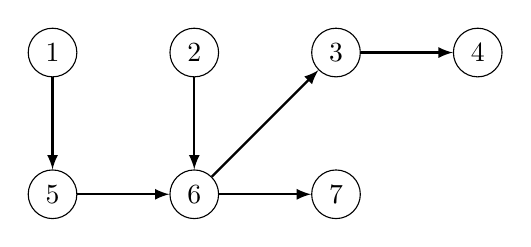
\begin{tikzpicture}[scale=0.9]
        \node[draw, circle] (1) at (0,0) {1};
        \node[draw, circle] (2) at (2,0) {2};
        \node[draw, circle] (3) at (4,0) {3};
        \node[draw, circle] (4) at (6,0) {4};
        \node[draw, circle] (5) at (0,-2) {5};
        \node[draw, circle] (6) at (2,-2) {6};
        \node[draw, circle] (7) at (4,-2) {7};

        \path[draw,thick,->,>=latex] (1) -- (5);
        \path[draw,thick,->,>=latex] (2) -- (6);
        \path[draw,thick,->,>=latex] (3) -- (4);
        \path[draw,thick,->,>=latex] (5) -- (6);
        \path[draw,thick,->,>=latex] (6) -- (3);
        \path[draw,thick,->,>=latex] (6) -- (7);
    \end{tikzpicture}
\end{center}

La cobertura de caminos general mínima de este grafo consiste de
dos caminos. Por ejemplo, el primer camino puede ser el siguiente:
\begin{center}
    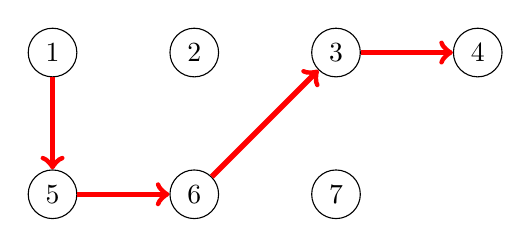
\begin{tikzpicture}[scale=0.9]
        \node[draw, circle] (1) at (0,0) {1};
        \node[draw, circle] (2) at (2,0) {2};
        \node[draw, circle] (3) at (4,0) {3};
        \node[draw, circle] (4) at (6,0) {4};
        \node[draw, circle] (5) at (0,-2) {5};
        \node[draw, circle] (6) at (2,-2) {6};
        \node[draw, circle] (7) at (4,-2) {7};

        \path[draw=red,thick,->,line width=2pt] (1) -- (5);
        \path[draw=red,thick,->,line width=2pt] (5) -- (6);
        \path[draw=red,thick,->,line width=2pt] (6) -- (3);
        \path[draw=red,thick,->,line width=2pt] (3) -- (4);
    \end{tikzpicture}
\end{center}
Y el segundo camino el siguiente:
\begin{center}
    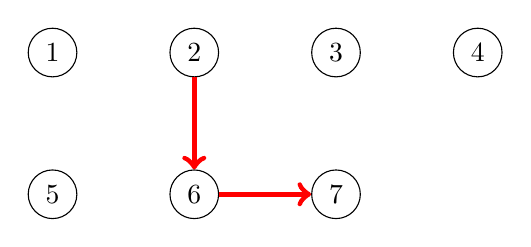
\begin{tikzpicture}[scale=0.9]
        \node[draw, circle] (1) at (0,0) {1};
        \node[draw, circle] (2) at (2,0) {2};
        \node[draw, circle] (3) at (4,0) {3};
        \node[draw, circle] (4) at (6,0) {4};
        \node[draw, circle] (5) at (0,-2) {5};
        \node[draw, circle] (6) at (2,-2) {6};
        \node[draw, circle] (7) at (4,-2) {7};

        \path[draw=red,thick,->,line width=2pt] (2) -- (6);
        \path[draw=red,thick,->,line width=2pt] (6) -- (7);
    \end{tikzpicture}
\end{center}

Una cobertura de caminos general mínima puede encontrarse casi como
una mínima cobertura de caminos disjunta en nodos. Es suficiente añadir
algunos nodos nuevos al grafo de matchings tal que haya una arista
$a \rightarrow b$ siempre y cuando haya un camino de $a \rightarrow b$
en el grafo original (posiblemente de múltiples aristas).

El grafo de matchings para el grafo de arriba es el siguiente:
\begin{center}
    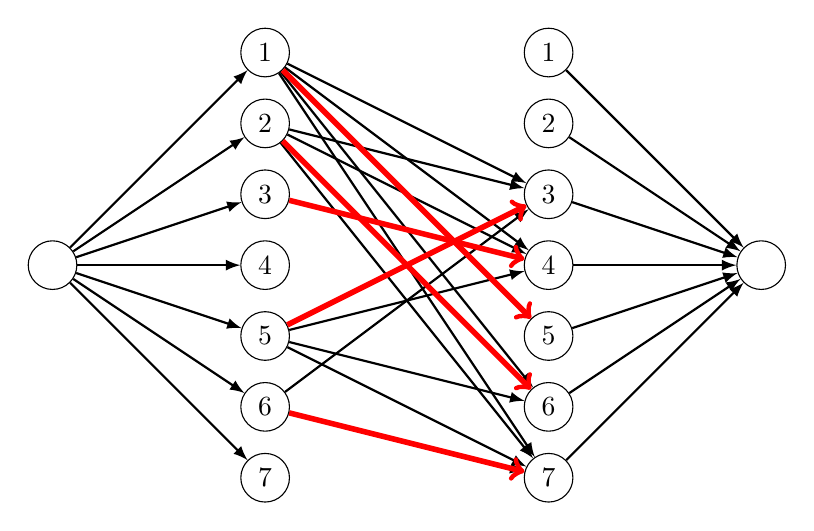
\begin{tikzpicture}[scale=0.9]
        \node[draw, circle] (1a) at (0,6) {1};
        \node[draw, circle] (2a) at (0,5) {2};
        \node[draw, circle] (3a) at (0,4) {3};
        \node[draw, circle] (4a) at (0,3) {4};
        \node[draw, circle] (5a) at (0,2) {5};
        \node[draw, circle] (6a) at (0,1) {6};
        \node[draw, circle] (7a) at (0,0) {7};

        \node[draw, circle] (1b) at (4,6) {1};
        \node[draw, circle] (2b) at (4,5) {2};
        \node[draw, circle] (3b) at (4,4) {3};
        \node[draw, circle] (4b) at (4,3) {4};
        \node[draw, circle] (5b) at (4,2) {5};
        \node[draw, circle] (6b) at (4,1) {6};
        \node[draw, circle] (7b) at (4,0) {7};

        \node[draw, circle] (a) at (-3,3) {\phantom{0}};
        \node[draw, circle] (b) at (7,3) {\phantom{0}};


        %\path[draw,thick,->,>=latex] (1a) -- (5b);
        \path[draw,thick,->,>=latex] (1a) -- (6b);
        \path[draw,thick,->,>=latex] (1a) -- (7b);
        \path[draw,thick,->,>=latex] (1a) -- (3b);
        \path[draw,thick,->,>=latex] (1a) -- (4b);
        \path[draw,thick,->,>=latex] (5a) -- (6b);
        \path[draw,thick,->,>=latex] (5a) -- (7b);
        %\path[draw,thick,->,>=latex] (5a) -- (3b);
        \path[draw,thick,->,>=latex] (5a) -- (4b);
        \path[draw,thick,->,>=latex] (6a) -- (7b);
        %\path[draw,thick,->,>=latex] (6a) -- (7b);
        \path[draw,thick,->,>=latex] (6a) -- (3b);
        %\path[draw,thick,->,>=latex] (3a) -- (4b);
        %\path[draw,thick,->,>=latex] (2a) -- (6b);
        \path[draw,thick,->,>=latex] (2a) -- (7b);
        \path[draw,thick,->,>=latex] (2a) -- (3b);
        \path[draw,thick,->,>=latex] (2a) -- (4b);


        \path[draw,thick,->,>=latex] (a) -- (1a);
        \path[draw,thick,->,>=latex] (a) -- (2a);
        \path[draw,thick,->,>=latex] (a) -- (3a);
        \path[draw,thick,->,>=latex] (a) -- (4a);
        \path[draw,thick,->,>=latex] (a) -- (5a);
        \path[draw,thick,->,>=latex] (a) -- (6a);
        \path[draw,thick,->,>=latex] (a) -- (7a);

        \path[draw,thick,->,>=latex] (1b) -- (b);
        \path[draw,thick,->,>=latex] (2b) -- (b);
        \path[draw,thick,->,>=latex] (3b) -- (b);
        \path[draw,thick,->,>=latex] (4b) -- (b);
        \path[draw,thick,->,>=latex] (5b) -- (b);
        \path[draw,thick,->,>=latex] (6b) -- (b);
        \path[draw,thick,->,>=latex] (7b) -- (b);

        \path[draw=red,thick,->,line width=2pt] (1a) -- (5b);
        \path[draw=red,thick,->,line width=2pt] (5a) -- (3b);
        \path[draw=red,thick,->,line width=2pt] (3a) -- (4b);
        \path[draw=red,thick,->,line width=2pt] (2a) -- (6b);
        \path[draw=red,thick,->,line width=2pt] (6a) -- (7b);


        % \path[draw=red,thick,->,line width=2pt] (1a) -- (6b);
        % \path[draw=red,thick,->,line width=2pt] (1a) -- (7b);
        % \path[draw=red,thick,->,line width=2pt] (1a) -- (3b);
        % \path[draw=red,thick,->,line width=2pt] (1a) -- (4b);
        % \path[draw=red,thick,->,line width=2pt] (5a) -- (6b);
        % \path[draw=red,thick,->,line width=2pt] (5a) -- (7b);
        % \path[draw=red,thick,->,line width=2pt] (5a) -- (3b);
        % \path[draw=red,thick,->,line width=2pt] (5a) -- (4b);
        % \path[draw=red,thick,->,line width=2pt] (6a) -- (7b);
        % \path[draw=red,thick,->,line width=2pt] (6a) -- (7b);
        % \path[draw=red,thick,->,line width=2pt] (6a) -- (3b);
        % \path[draw=red,thick,->,line width=2pt] (3a) -- (4b);
        % \path[draw=red,thick,->,line width=2pt] (2a) -- (6b);
        % \path[draw=red,thick,->,line width=2pt] (2a) -- (7b);
        % \path[draw=red,thick,->,line width=2pt] (2a) -- (3b);
        % \path[draw=red,thick,->,line width=2pt] (2a) -- (4b);

    \end{tikzpicture}
\end{center}

\subsubsection{Teorema de Dilworth}

\index{teorema de Dilworth}
\index{anticadena}

Una \key{anticadena} es un conjunto de nodos de un grafo tal que
no exista un camino de un nodo a otro utilizando aristas del grafo.
El \key{teorema de Dilworth} establece que en un grafo acíclico dirigido,
el tamaño de una cobertura de caminos general mínima es igual al tamaño
de una anticadena máxima.

Por ejemplo, los nodos 3 y 7 forman una anticadena en el siguiente grafo:

\begin{center}
    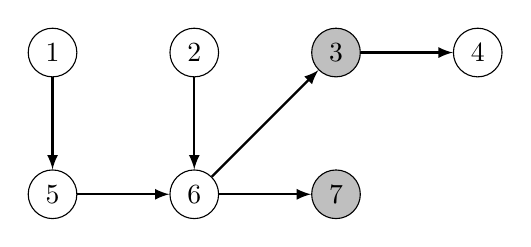
\begin{tikzpicture}[scale=0.9]
        \node[draw, circle] (1) at (0,0) {1};
        \node[draw, circle] (2) at (2,0) {2};
        \node[draw, circle, fill=lightgray] (3) at (4,0) {3};
        \node[draw, circle] (4) at (6,0) {4};
        \node[draw, circle] (5) at (0,-2) {5};
        \node[draw, circle] (6) at (2,-2) {6};
        \node[draw, circle, fill=lightgray] (7) at (4,-2) {7};

        \path[draw,thick,->,>=latex] (1) -- (5);
        \path[draw,thick,->,>=latex] (2) -- (6);
        \path[draw,thick,->,>=latex] (3) -- (4);
        \path[draw,thick,->,>=latex] (5) -- (6);
        \path[draw,thick,->,>=latex] (6) -- (3);
        \path[draw,thick,->,>=latex] (6) -- (7);
    \end{tikzpicture}
\end{center}

Esta es una anticadena máxima, porque no es posible construir una
anticadena que contuviera tres nodos. Hemos visto anteriormente que
el tamaño de una cobertura de caminos general mínima de este grafo
consiste de dos caminos.
